% Transaction Anatomy Diagram
% Visual breakdown of all transaction components with size annotations
%
% ACCESSIBILITY ALT TEXT:
% A structural diagram showing the components of a Botho transaction. The
% main box contains: Header (32 bytes) at top, Inputs section (each 680
% bytes with ring references and key image), Outputs section (each 1152
% bytes with commitment, stealth key, and KEM ciphertext), CLSAG signatures
% (704 bytes per input), and Bulletproof range proof (736 bytes aggregated).
% Total transaction size is approximately 4.5 KB for a typical 1-input,
% 2-output transaction.

\begin{figure}[ht]
\centering
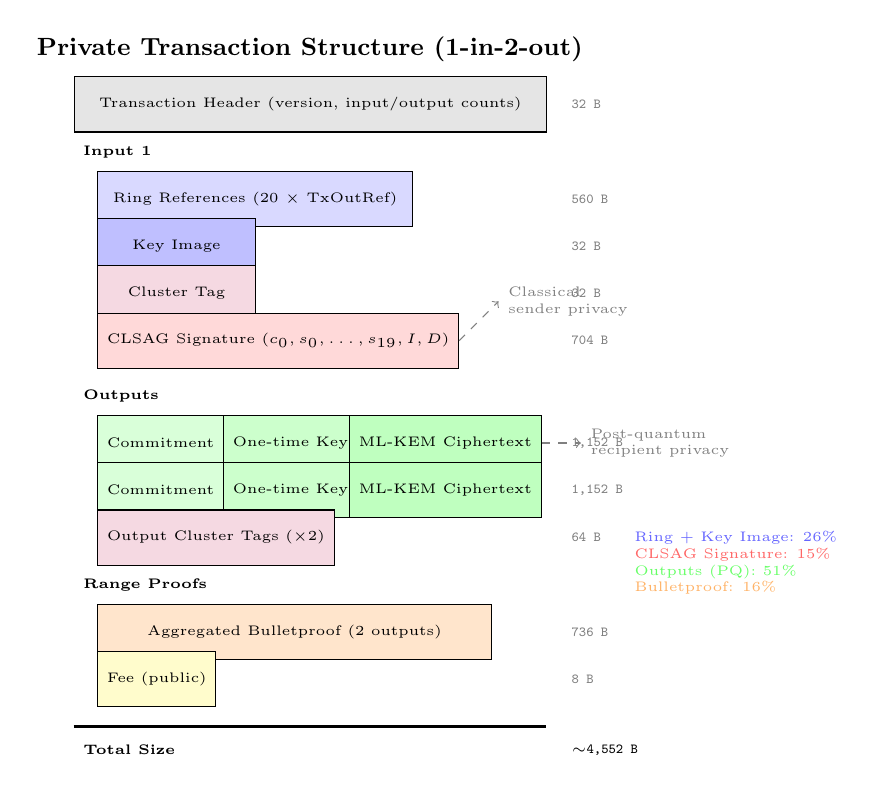
\begin{tikzpicture}[
    component/.style={draw, rectangle, minimum height=0.7cm, font=\tiny, anchor=west},
    label/.style={font=\tiny, anchor=east},
    size/.style={font=\tiny\ttfamily, anchor=west, text=gray}
]
    % Title
    \node[font=\small\bfseries] at (3,5.5) {Private Transaction Structure (1-in-2-out)};

    % Header section
    \node[component, fill=gray!20, minimum width=6cm] (header) at (0,4.8) {Transaction Header (version, input/output counts)};
    \node[size] at (6.2,4.8) {32 B};

    % Input section header
    \node[font=\tiny\bfseries, anchor=west] at (0,4.2) {Input 1};

    % Ring references
    \node[component, fill=blue!15, minimum width=4cm] (ring) at (0.3,3.6) {Ring References (20 $\times$ TxOutRef)};
    \node[size] at (6.2,3.6) {560 B};

    % Key image
    \node[component, fill=blue!25, minimum width=2cm] (keyimg) at (0.3,3.0) {Key Image};
    \node[size] at (6.2,3.0) {32 B};

    % Cluster tag (input)
    \node[component, fill=purple!15, minimum width=2cm] (intag) at (0.3,2.4) {Cluster Tag};
    \node[size] at (6.2,2.4) {32 B};

    % CLSAG signature
    \node[component, fill=red!15, minimum width=4.5cm] (clsag) at (0.3,1.8) {CLSAG Signature ($c_0, s_0, \ldots, s_{19}, I, D$)};
    \node[size] at (6.2,1.8) {704 B};

    % Output section header
    \node[font=\tiny\bfseries, anchor=west] at (0,1.1) {Outputs};

    % Output 1
    \node[component, fill=green!15, minimum width=1.5cm] (out1com) at (0.3,0.5) {Commitment};
    \node[component, fill=green!20, minimum width=1.5cm] (out1key) at (1.9,0.5) {One-time Key};
    \node[component, fill=green!25, minimum width=2cm] (out1kem) at (3.5,0.5) {ML-KEM Ciphertext};
    \node[size] at (6.2,0.5) {1,152 B};

    % Output 2
    \node[component, fill=green!15, minimum width=1.5cm] (out2com) at (0.3,-0.1) {Commitment};
    \node[component, fill=green!20, minimum width=1.5cm] (out2key) at (1.9,-0.1) {One-time Key};
    \node[component, fill=green!25, minimum width=2cm] (out2kem) at (3.5,-0.1) {ML-KEM Ciphertext};
    \node[size] at (6.2,-0.1) {1,152 B};

    % Output cluster tags
    \node[component, fill=purple!15, minimum width=3cm] (outtags) at (0.3,-0.7) {Output Cluster Tags ($\times$2)};
    \node[size] at (6.2,-0.7) {64 B};

    % Bulletproof section
    \node[font=\tiny\bfseries, anchor=west] at (0,-1.3) {Range Proofs};

    \node[component, fill=orange!20, minimum width=5cm] (bp) at (0.3,-1.9) {Aggregated Bulletproof (2 outputs)};
    \node[size] at (6.2,-1.9) {736 B};

    % Fee
    \node[component, fill=yellow!20, minimum width=1.5cm] (fee) at (0.3,-2.5) {Fee (public)};
    \node[size] at (6.2,-2.5) {8 B};

    % Total bar
    \draw[thick] (0,-3.1) -- (6,-3.1);
    \node[font=\tiny\bfseries, anchor=west] at (0,-3.4) {Total Size};
    \node[font=\tiny\ttfamily\bfseries, anchor=west] at (6.2,-3.4) {$\sim$4,552 B};

    % Size breakdown pie-style annotation
    \node[font=\tiny, align=left, anchor=north west] at (7,-0.5) {
        \textcolor{blue!60}{Ring + Key Image: 26\%}\\
        \textcolor{red!60}{CLSAG Signature: 15\%}\\
        \textcolor{green!60}{Outputs (PQ): 51\%}\\
        \textcolor{orange!60}{Bulletproof: 16\%}
    };

    % Annotation arrows
    \draw[->, gray, dashed] (out1kem.east) -- ++(0.5,0) node[right, font=\tiny, align=left] {Post-quantum\\recipient privacy};

    \draw[->, gray, dashed] (clsag.east) -- ++(0.5,0.5) node[right, font=\tiny, align=left] {Classical\\sender privacy};

\end{tikzpicture}
\caption{Anatomy of a private transaction (1 input, 2 outputs). The ML-KEM
ciphertext dominates output size (1,088 bytes each) but provides post-quantum
recipient privacy. Ring signatures use classical CLSAG for efficiency. Total
size is approximately 4.5 KB, compared to $\sim$50 KB with post-quantum ring
signatures.}
\label{fig:tx-anatomy}
\end{figure}
